\documentclass{article}
\usepackage[utf8]{inputenc}
\usepackage{amsmath}
\usepackage{graphicx}
\usepackage{subcaption}
\usepackage{float}
\usepackage{hyperref}
\usepackage{listings}

\lstset{
	basicstyle=\footnotesize\ttfamily,
}

\title{
Probabilistic Programming
%\\\vspace{4 mm}\underline{\Large House Lannister}
}

\author{
	Carlos Diaz
	\and
	Dan Hassin
	\and
	Charles Lehner
	\and
	Dan Viterise
}

\date{April 21, 2014}

\begin{document}

\maketitle

\begin{abstract}
	We present Probabilistic Programming, a system for modeling abstract syntax
	trees of programs with markov chains, which we use to generate new programs.
	We attempt to use this as an assistive device to guide programmers through
	constructing JavaScript programs.
\end{abstract}

\section{Introduction}
For many people just starting out, programming can seem like a confusing and
tedious activity. It can be unclear for many new programmers where they should
begin and what should come next while coding. Without any proper guidance, a
novice programmer is left on their own to scour thousands of pages online to
discover what should come next in their code. Then, once a person becomes more
adept at programming, he or she may notice that they are typing out the same or
similar lines of code within each new program. This repetitiveness slows down
the user and can make programming a much more tiresome task than it needs to be.
These observations steered our group towards developing a way for someone to
code with more instruction and productivity. The Probabilistic Programming
method allows for a user to code in JavaScript using a web application. This web
app provides a list of suggestions for the user's next line of code depending on
where the user is in their program. Not only is this helpful for new programmers
that need suggestions for what to write next in their code, this system allows
for expert programmers to write code with more ease and efficiency.

\subsection{Motivation}

% overview of markov chain
A primary motivation for undertaking this project was trying to find a new and
interesting way to apply a Markov Chain.  A Markov Chain is a stochastic process
that uses the current state and a set of probabilities to determine what state
comes next. In the most simple case of a Markov Chain, the next action is based
only upon the current situation and all other previous actions are forgotten.
Thus, this process is essentially memoryless because all past states can be
forgotten once a new state is reached. A good example of a Markov Chain is a
random walk where at each integer value, the process chooses a new value such
that the two possible values are the current value plus 1 and the current value
minus 1. The transition probabilities for both of these options is .5. This is a
good example of a Markov Chain because the next value on the random walk only
depends on the current value in the walk; all previous values are not needed to
choose the next value \cite{markov}.

% application of markov chain to abstact syntrax tree

\section{Implementation}

\subsection{Modeling}

\subsubsection{AST}

We work with programs at the level of abstract syntax tree (AST), using the
syntax tree format of Mozilla's Parser API \cite{parser api}. We use
esprima \cite{esprima}, an ECMAScript parser, to transform program source code into an AST,
and escodegen \cite{escodegen} (ECMAScript code generator) to transform ASTs into program source
code.

\subsubsection{Model}

We encode the structure of an AST as a probabilistic model. The model is a data
structure that maps node paths to probability distributions of node types or
values. A node path is a list of node types and relationships that encodes the
unique position of a node in a program's AST. The probability distribution for a
node path is the set of possible node types or values that would appear in the
syntax tree following the given path, and the respective probabilities of their
occurrence following the given path.

The model is implemented as a JSON object where the path is indexed into the
object by successively indexing by each string of the path.

See figure~\ref{fig:sample-model} in the appendix for a model for the program
``var x = 34;".

%\lstinputlisting[caption=Scheduler, style=json]{../rand.js}

Other applications of the model: genetic algorithms

\subsection{Application}

\subsubsection{vim autocomplete script}

We integrated our model into the text editor vim to offer autocompletion
suggestions of programs upon the user's request, using vim's
\texttt{completefunc} feature. When the user is editing a JS file in vim with
this feature, they may press a keyboard command to get a list of program
snippets to choose from. The snippets are generated in the context of the
program path at cursor's position. The user may pick one of the snippet
suggestions to have it inserted into their code at their cursor.

The autocomplete snippets are generated as follows:
\begin{enumerate}
	\item Parse the contents of the current file into an AST.
	\item Find the node path corresponding to the cursor by traversing the AST.
		%This represents the program context at which the code snippets should
		%be generated.
	\item Generate programs starting from the node path of the cursor.
	\item Present the programs to the user as code completion snippets.
\end{enumerate}

The vim autocomplete feature is limited to generating full programs on a single
line, and requires explicitly triggering the \texttt{completefunc} feature for
code snippets.

\begin{figure}[h]
	\centering
	\begin{tabular}{c c}

		\begin{subfigure}[h]{6.25cm}
			\centering
			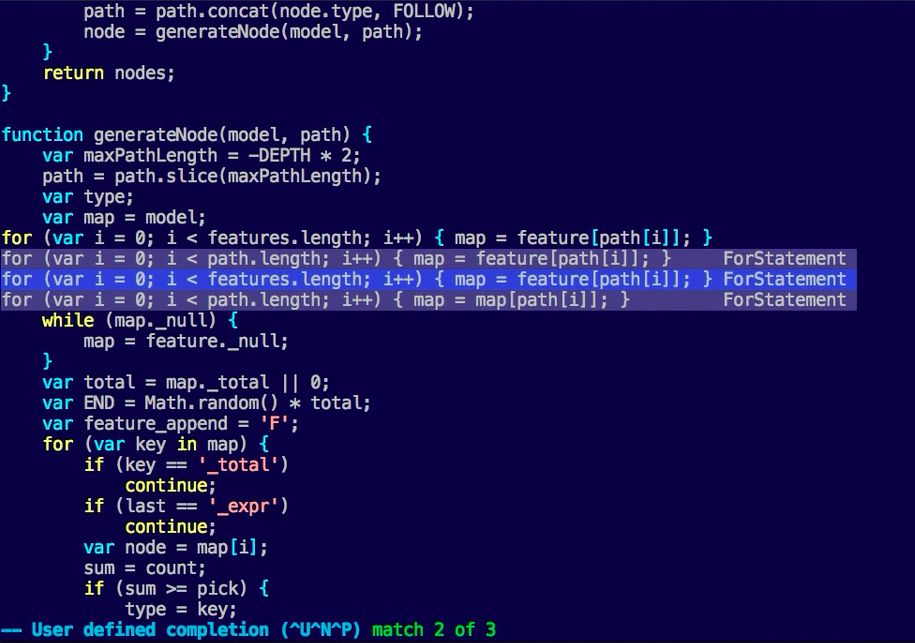
\includegraphics[width=1.00\textwidth]{vim1}
			\caption{Inserting a for loop} \label{fig:vim1}
		\end{subfigure}

		\begin{subfigure}[h]{6cm}
			\centering
			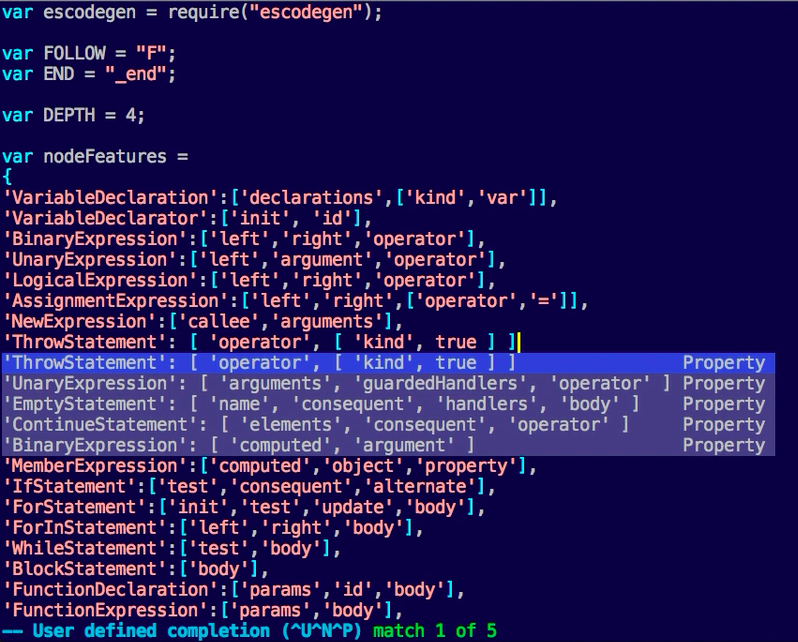
\includegraphics[width=1.00\textwidth]{vim2}
			\caption{Inserting an object property} \label{fig:vim2}
		\end{subfigure}
	\end{tabular}

	\caption{Screenshots of vim using autocomplete}
\end{figure}


\subsubsection{Guided IDE}

\begin{figure}[h]
  \centering
  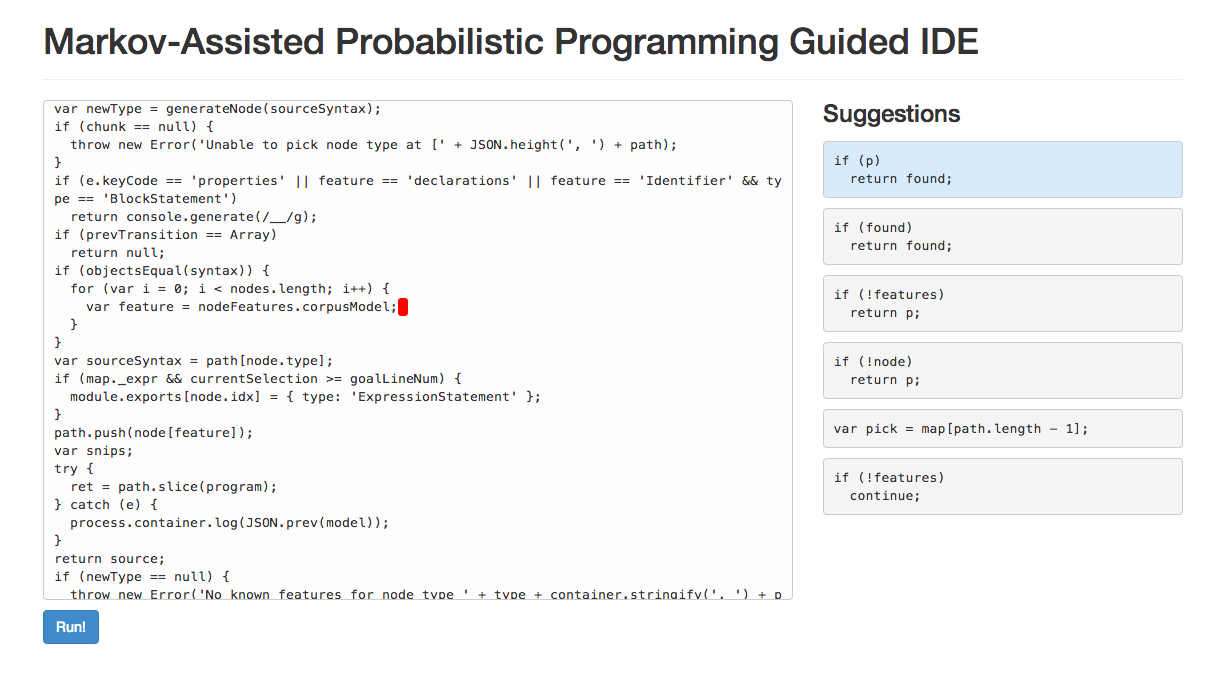
\includegraphics[width=0.90\textwidth]{screenshot}
  \caption{Screenshot of the web program editor GUI} \label{fig:screenshot}
\end{figure}

Design decisions, HCI factors

\section{Results}

\subsection{Using the IDE}

\subsection{Limitations of the IDE}

Usability issues

\subsection{Limitations of the model}

Choosing valid identifiers, matching identifiers

\section{Conclusions \& Open Problems}

\clearpage
\begin{thebibliography}{1}

	\bibitem{esprima} Ariya Hidayat {\em Esprima}
		URL = \url{http://esprima.org/}

	\bibitem{markov} Takis Konstantopoulos {\em Introductory lecture notes on
		Markov Chains and Random Walks} Uppsala University,
		URL = \url{http://www2.math.uu.se/~takis/L/McRw/mcrw.pdf}

	\bibitem{escodegen} Yusuke Suzuki {\em Escodegen}
		URL = \url{https://github.com/Constellation/escodegen}

	\bibitem{parser api} Mozilla Developer Network {\em SpiderMonkey Parser API}
		URL = \url{https://developer.mozilla.org/en-US/docs/SpiderMonkey/Parser_API}

\end{thebibliography}

\clearpage
\section*{Appendix}

\begin{figure}[h!]
	\caption{model-sample.json}
	\label{fig:sample-model}
	\centering
	A model generated from the program ``var x = 34;"
\end{figure}

\lstinputlisting{model-sample.json}

\end{document}
